\section{Bayes' Theorem and Limit Setting} \label{sec:fit:theory}

In the Bayesian approach, the data are considered to be fixed and a probability
is assigned to the parameters of the theory. Thus, given the data, a
probability is assigned to the number of signal events which could be present
in the data.  In other words, Bayes' theorem enables us to calculate the
conditional probability of event $A$, the parameters of the theory, occurring
given that event $B$, the data, has occurred. This is given by 

\begin{equation} \label{sec:fit:general_bayes} 
P(A|B) = \frac{P(B|A)P(A)}{P(B)}, 
\end{equation}

where $P(B|A)$ is the conditional probability of event $B$ occuring, given that
event $A$ has occurred, $P(A)$ is the probability of event $A$ occuring, and
$P(B)$ is the probability of event $B$ occuring. For events where the outcome
is continuous rather than discrete, the probabilities ($P$) are replaced by
probability density functions ($p$ or p.d.f).

In this analysis the parameters of the theory are the normalization of the
signal template $\nu$, which is equivalent to the number of signal events, and
the nuisance parameters $\boldsymbol{\theta}$, which are the systematics
discussed in \Cref{chap:systematics}. Utilizing the continuous form of Bayes'
theorem given in \Cref{sec:fit:general_bayes} the p.d.f can be calculated for
the theory parameters ($\nu,\boldsymbol{\theta}$), given the data.  This
particular p.d.f is referred to as the posterior as it reflects the knowledge
about the theory parameters after the data has been analyzed and is given in
\Cref{eq:fit:posterior}.

\begin{equation} \label{eq:fit:posterior}
p(\nu,\boldsymbol{\theta}|\text{Data}) = \frac{\mathcal{L}(\nu,\boldsymbol{\theta}|\text{Data})\pi(\nu,\boldsymbol{\theta})}{p(\text{Data})}
\end{equation}

Here the likelihood of the theory parameters, given the data, is denoted
$\mathcal{L}(\nu,\boldsymbol{\theta}|\text{Data})$ and is equivalent to
$p(\text{Data}|\nu,\boldsymbol{\theta})$.  The exact form of the likelihood is
a choice of the analyzer and is discussed further in \Cref{sec:fit:bat}. The
information known about the theory parameters before the data is analyzed is
contained in the prior probability density $\pi(\nu,\boldsymbol{\theta})$.
This can be re-written as $\pi(\nu,\boldsymbol{\theta}) =
\pi(\nu)\prod_{i}\pi(\theta_i)$ since the parameter of interest $\nu$ and each
of the nuisance parameters $\theta_i$ are independent from eachother.  The form
of the priors for the signal and each systematic is chosen by the analyzer and
is discussed in \Cref{sec:fit:priors}.  Note that the denominator of
\Cref{eq:fit:posterior}, $p(\text{Data})$, is simply an overall normalization
factor and therefore can be dropped during the limit seting procedure.

The ultimate goal is to obtain the p.d.f for a single parameter, the number of
signal events $\nu$, given the data.  This is known as the marginalized
posterior $p(\nu|\text{Data})$.  This is done by integrating out the dependence
of \Cref{eq:fit:posterior} on $\boldsymbol{\theta}$ as shown in
\Cref{eq:fit:marginalization}.

\begin{equation} \label{eq:fit:marginalization}
p(\nu|\text{Data}) = \int p(\nu,\boldsymbol{\theta}|\text{Data})\text{d}\boldsymbol{\theta}
\end{equation}

This multi-dimentional intergral over the nuisance parameters is known as
marginalization.  Note that the space of nuisance parameters may be very large,
making this intergral extremely computationally expensive to calculate.  To
expedite this process a Markov Chain Monte Carlo procedure is implemented as
discussed in \Cref{sec:fit:bat}. By substituting the definition of the
posterior (\Cref{eq:fit:posterior}) into the marginalized posterior
(\Cref{eq:fit:marginalization}), utilizing the expanded prior probability
density $\pi(\nu,\boldsymbol{\theta}) = \pi(\nu)\prod_{i}\pi(\theta_i)$ and
dropping the $p(\text{Data})$ normalization factor gives the following
definition of Bayes' equation: 

\begin{equation} \label{eq:fit:bayes}
p(\nu|\text{Data}) \propto \int \mathcal{L}(\nu,\boldsymbol{\theta}|\text{Data})\pi(\nu)\prod_{i}\pi(\theta_i)\text{d}\boldsymbol{\theta}
\end{equation}

This form of Bayes' equation can be interpreted as follows: the prior knowledge
of the analyzer encoded into $\pi(\nu)$ and $\pi(\theta_{i})$, is updated by
the outcome of the experiment contained in the likelihood
$\mathcal{L}(\nu,\boldsymbol{\theta}|\text{Data})$ by marginalizing the
posterior w.r.t $\boldsymbol{\theta}$ in order to obtain the p.d.f of the
parameter of interest given the data, $p(\nu|\text{Data})$.  This is shown
diagramatically for the simlified case neglecting nuisance parameters for a
small data sample in \Cref{fig:fit:small_data} and a large data sample in
\Cref{fig:fit:big_data} both with a flat signal prior.  The flat prior in
these figures represents an uninformative prior to reflect ignorance about
the value of the parameter such that it has minimal influence on the obtained
posterior.  This choice is consistent with similar dijet analysis
\cite{Beresford:2642397} and simplifies the comparison of results.

\begin{figure}[!htbp]
\centering
\subcaptionbox{\label{fig:fit:small_data}}{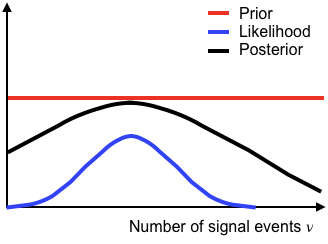
\includegraphics[width=0.49\linewidth]{figures/fit/small_data}} \hfill
\subcaptionbox{\label{fig:fit:big_data}}{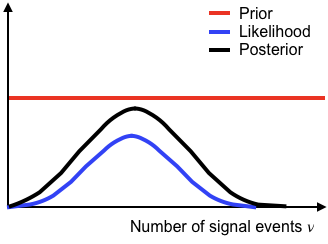
\includegraphics[width=0.49\linewidth]{figures/fit/big_data}}
\caption{Cartoon representing the relationship between the signal normalization prior $\pi(\nu)$ (red), likelihood $\mathcal{L}(\nu|\text{Data})$ (blue), and posterior $p(\nu|\text{Data})$ (black) for the cases of (a) a small data sample and (b) a larger data sample.  This simplified example contains no nuisance parameters.}
\label{sec:fit:marginalization}
\end{figure}

By integrating the marginalized posterior $p(\nu|\text{Data})$ across a range
of $\nu$ values the probability that the true value of $\nu$ lies in the chosen
region can be determined.  A common choice in particle physics is to define the
upper limit $\nu_{\text{upper}}$ as the value below which 95\% of the marginalized
posterior lies, referred to as the 95\% credibility level (CL) as shown in
equation \Cref{eq:fit:limit} below.

\begin{equation} \label{eq:fit:limit}
0.95 = \int_{-\infty}^{\nu_{\text{upper}}} p(\nu|\text{Data}) \text{d}\nu
\end{equation}

Here p(\nu|\text{Data}) is given by \Cref{eq:fit:bayes}. This means there is a
95\% probability that the number of signal events in the data is equal to
$\nu_{\text{upper}}$ or fewer.  This definition is used in the final fit to
define the 95\% CL.


